\section{Method}\label{sec:Method}

We have collected endpoints from ten different REST APIs and implemented the detection algorithms for linguistic and design quality based on the literature. 

We have created a Node.js program for making HTTP requests to the selected API endpoints and check for REST design antipatterns. For detecting linguistic patterns and antipatterns the Java program created by Palma et al. for their study of linguistic REST antipatterns \cite{linguistic} for checking for those types of patterns and antipatterns in the endpoints was used. 

To answer RQ1 we have performed a Chi-Square test on the design quality data \textit{vs.} the linguistic quality data, see table \ref{contingencytable} for more about the Chi-Square test. To answer the other research questions, we have performed pairwise Phi coefficient analyses. Figure \ref{fig:Methodfigure} below illustrates our overall research method. 

\begin{figure}[ht!]
 \centering
 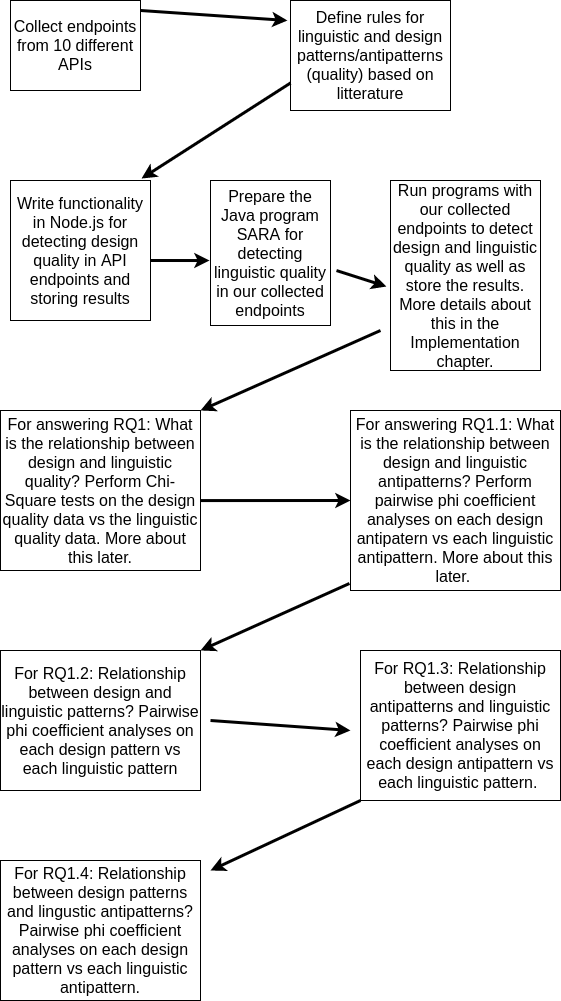
\includegraphics[scale=0.5]{img/method_figures/method_figure.png}
 \caption{Our research methodology.}
 \label{fig:Methodfigure}
\end{figure}



\subsection{APIs Used for the Study}

We selected ten REST APIs for this study. In Table \ref{tab:APIsusedintheresearch}, each API is listed with their current version in use and link to documentation.

\begin{center}
\begin{table}[!ht]
\small
\begin{tabular}{|p{25mm}|p{12mm}|p{100mm}|}
\hline \textbf{APIs} & \textbf{Version} & \textbf{Documentation} \\
\hline 
Facebook &
7.0 & 
\url{https://developers.facebook.com/docs/apis-and-sdks/} 
\\ \hline
Nasa &
- &
\url{https://ssd-api.jpl.nasa.gov/doc/index.php}
\\ \hline
Imgur &
3 & 
\url{https://apidocs.imgur.com/?version=latest}
\\ \hline
Disqus &
3 & 
\url{https://disqus.com/api/docs/}
\\ \hline
GitHub &
- & 
\url{https://developer.github.com/v3/}
\\ \hline
Twitter &
1.1 & 
\url{https://developer.twitter.com/en}
\\ \hline
Bitly &
3 & 
\url{https://dev.bitly.com/}
\\ \hline
StackExchange &
2.2 & 
\url{https://api.stackexchange.com/}
\\ \hline
Vimeo &
3 & 
\url{https://developer.vimeo.com/}
\\ \hline
Spotify &
1 & 
\url{https://developer.spotify.com/documentation/}
\\ \hline
\end{tabular}
 \caption{The list of REST APIs used in the study.}
 \label{tab:APIsusedintheresearch}
\end{table}
\end{center}

\subsection{REST Design Antipatterns}

Based on the research about REST design quality conducted by Palma et al. \cite{design}, we identify six REST design antipatterns and rules for their detection in this study. Table \ref{tab:RulesfordetectingRESTdesignantipatterns} list each antipattern with their rule for detection.

\begin{table}[!ht]
\begin{center}
\small
\begin{tabular}{|p{5cm}|p{9cm}|}
\hline \textbf{Name} & \textbf{Rules} \\
\hline 
Breaking Self-descriptiveness &
When a request or response contains non-standard headers \cite{design}. Figure \ref{fig:BreakingSelf-descriptiveness} shows our implementation of this detection.


\\ \hline
Forgetting Hypermedia &
When the response body of a GET request does not contain links to relevant resources or when the response of a POST request does not contain that or a Location header \cite{design}. Figure \ref{fig:ForgettingHypermedia} shows our implementation of this detection.

\\ \hline
Ignoring Caching &
When a response of a GET request does not contain an ETag or the request or response headers do not contain a Cache-Control header or that is set to no-cache or no-store \cite{design}. Figure \ref{fig:IgnoringCaching} shows our implementation of this detection.

\\ \hline
Ignoring MIME Types &
When a response's Content-Type header's value is not a standard MIME type or if it is not among the accepted MIME types requested \cite{design}. Figure \ref{fig:IgnoringMIMETypes} shows our implementation of this detection.

\\ \hline
Ignoring Status Code &
When the combination of HTTP method, status code, and status text is not a valid combination \cite{design}. Figure \ref{fig:IgnoringStatusCode} shows our implementation of this detection.

\\ \hline
Misusing Cookies &
When the request or response contains any kind of cookie header \cite{design}. Figure \ref{fig:MisusingCookies} shows our implementation of this detection.

\\ \hline
\end{tabular}
 \caption{Rules for detecting REST design antipatterns based on SOFA.}
 \label{tab:RulesfordetectingRESTdesignantipatterns}
 \end{center}
\end{table}

\clearpage

\subsection{REST Design Patterns}
Based on the research about REST Design Quality conducted by Palma et al. \cite{design}, three design patterns are identified and used in the study. In Table \ref{tab:RulesforRESTdesignpatterns} they are listed together with rule for detection.

\begin{center}
\begin{table}[!ht]
\small
\begin{tabular}{|p{5cm}|p{9cm}|}
\hline \textbf{Name} & \textbf{Rules} \\
\hline 
Content Negotiation &
When the value of a response’s Content-Type header is a standard MIME type and among the accepted MIME types requested \cite{design}. This is the corresponding pattern to the Ignoring MIME types antipattern.

\\ \hline
Entity Linking &
When the response body of a GET request contains links to relevant resources or when the response of a POST request contains that or a Location header \cite{design}. This is the corresponding pattern to the Forgetting Hypermedia antipattern. 

\\ \hline
Response Caching &
When a response to a GET request contains an ETag or when the request or response headers contain a Cache-Control header which is not set to no-cache or no-store \cite{design}. This is the corresponding pattern to the  Ignoring Caching antipattern. 

\\ \hline
\end{tabular}
 \caption{Rules for REST design patterns based on SOFA.}
 \label{tab:RulesforRESTdesignpatterns}
\end{table}
\end{center}

\subsection{Linguistic Antipatterns}

Based on the research about REST linguistic quality conducted by Palma et al. \cite{linguistic}, five linguistic antipatterns are defined in the study. In Table \ref{tab:Rulesforlinguisticantipatterns}, they are listed with rule for detection.
\begin{center}
\begin{table}[!ht]
\small
\begin{tabular}{|p{30mm}|p{105mm}|}
\hline \textbf{Name} & \textbf{Rules} \\
\hline 
Contextless Resource Names &
When the words in the URI nodes are not within the same context \cite{linguistic}. \newline Antipattern example: example.com/mammals/pigeons\\ \hline
Non-hierarchical Nodes &
When the URI nodes are not in a hierarchical order \cite{linguistic}. \newline Antipattern example: example.com/squirrels/mammals\\ \hline
Amorphous URIs &
When the URI nodes contain symbols that hinder readability like underscores, upper case letters for anything other than the first letter, trailing slashes or file extensions \cite{linguistic}. \newline Antipattern example: 
example.com/small\_mammals/Squirrel5\\ \hline
CRUDy URIs &
When the URI contains words that indicate the action its request performs. Instead, the action performed should be determined by which HTTP method is used \cite{linguistic}. \newline Antipattern example: 
example.com/update-animal/mammals/squirrels?id=5\\ \hline
Pluralised Nodes
&
When the HTTP method is PUT or DELETE and the last node is a plural word. Or when the HTTP method is POST and the last node is not a plural word \cite{linguistic}. \newline Antipattern examples: PUT example.com/animals/squirrels and POST example.com/animals/squirrel

\\ \hline
\end{tabular}
 \caption{Rules for linguistic antipatterns based on SOFA.}
 \label{tab:Rulesforlinguisticantipatterns}
\end{table}
\end{center}

\clearpage

\subsection{Linguistic Patterns}

Linguistic patterns will be treated as linguistic antipatterns in reverse. In other words, if an antipattern is not detected it will be considered as the corresponding  pattern. Table \ref{tab:Rulesforlinguisticpatterns} describe each pattern and rule for its detection, based on the research on REST linguistic quality conducted by Palma et al. \cite{linguistic}.

\begin{center}
\begin{table}[!ht]
\small
\begin{tabular}{|p{30mm}|p{105mm}|}
\hline \textbf{Name} & \textbf{Rules} \\
\hline 
Contextualised Resource Names &
When the words in the URI nodes are within the same context \cite{linguistic}. This is the corresponding pattern of Contextless Resource Names. \newline Pattern example: 
example.com/mammals/squirrels\\ \hline
Hierarchical Nodes &
When the URI nodes are in a proper and logical hierarchical order \cite{linguistic}. This is the corresponding pattern of Non-hierarchical Nodes. \newline Pattern example: /house/room/door\\ \hline
Tidy URIs &
When the URI nodes do not contain symbols that hinder readability \cite{linguistic}. This is the corresponding pattern of Amorphous URIs.\\ \hline
Verbless URIs &
When the URI does not contain words that indicate the action its request performs. And when instead, the action performed is determined by which HTTP method is used \cite{linguistic}. This is the corresponding pattern of CRUDy URIs. \newline Pattern example: 
PUT example.com/mammals/squirrel\\ \hline
Singularised Nodes
&
When the HTTP method is PUT or DELETE and the last node is a singular word. Or when the HTTP method is POST and the last node is not a singular word \cite{linguistic}. This is the corresponding pattern of the Pluralised Nodes antipattern. \newline Pattern examples: PUT example.com/animals/squirrel and POST example.com/animals/squirrels\\ \hline
\end{tabular}
 \caption{Rules for linguistic patterns based on SOFA.}
 \label{tab:Rulesforlinguisticpatterns}
\end{table}
\end{center}

\clearpage

\subsection{Reliability and Validity} \label{Reliability and Validity}

To increase the reliability, our study includes several appendixes, for example, links to repositories/downloads of the source code used (with documentation for how to use it), as well as a document of all the API endpoints used. This will make it possible for others to recreate and inspect the research conducted. Unit tests are exists for the antipattern detection methods in the Node.js program for detecting REST design antipatterns. 
One reliability risk is that the API versions used might become outdated and replaced with new versions. The API versions used have therefore been listed to let future researchers that might want to replicate our findings know which API versions were used. Hopefully the API versions we used will still be supported.

Another reliability risk is that the APIs could fix some errors detected which could produce different results if the detection programs used in this study are used again in the future. However, large changes within an API version should be unlikely. 
The biggest challenge will be to achieve a high validity. Time is a limited resource, there are limits to the amount of APIs that can be inspected and how many endpoints can be inspected in those. The  selection of APIs will be based on previous research by Palma et al. \cite{linguistic} and Google APIs will be excluded from them. From those APIs endpoints will be prioritized that have unique qualities and are prominent in the documentation. 

Another threat to validity is that our findings might become less relevant if the problems found are fixed in later versions. However, even if the results would become significantly different in future versions, the result of this study would still provide a snapshot of current conditions. 

\clearpage
\newpage